\documentclass[12pt]{article}
\usepackage[utf8]{inputenc}
\usepackage[czech]{babel}
\usepackage[T1]{fontenc}
\usepackage{hyperref}
\usepackage{epstopdf}

\newcommand{\HRule}{\rule{\linewidth}{0.5mm}}
\newcommand{\noun}[1]{\textsc{#1}}
\newcommand{\code}[1]{\texttt{#1}}
\newcommand{\cmake}{\noun{CMake} }
\newcommand{\fakeinput}{\noun{FakeInput} }

\begin{document}
\begin{titlepage}

\begin{center}

\textsc{\normalsize
    Zápočtová práce z předmětu\\
    Java (NPRG013)\\
    MFF UK
}\\[1.5cm]


% Title
\HRule \\[0.4cm]
{\huge \bfseries Colos}

\HRule \\[1.5cm]

\textsc{\Large Uživatelská dokumentace}\\[2cm]

% Author and supervisor
%\begin{minipage}{0.4\textwidth}
%\begin{flushleft} \large
\emph{Autor:}\\
Richard Jedlička
%\end{flushleft}
%\end{minipage}

\vfill

% Bottom of the page
{\large \today}

\end{center}

\end{titlepage}


\tableofcontents
\newpage

\section{Úvod}
Colos je aplikace určená pro výběr barvy. Umožnuje vabírat barvu v několika barevných modelech - RGB, HSL, HSV. Parametry barvy lze upravovat buď myší pomocí posuvníků, nebo číselně.

\section{Používání}
    \subsection{RGB model}
    \begin{figure}[!htb]
\centering
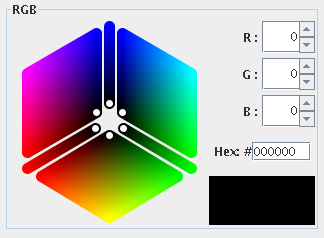
\includegraphics[scale=0.7]{rgb}
\caption{Digraph.}
\label{fig:digraph}
\end{figure}
    Pro použití knihovny ve Vaší aplikaci stačí na\code{inkludovat} potřebné hlavičkové soubory a při kompilaci knihovnu přilinkovat.

    Dále bude popsána stručně základní práce s jednotlivými hlavičkovými soubory.
    Konkrétní detaily lze nalézt v API dokumentaci, kterou lze vygenerovat při sestavování. Případně lze vše dohledat přímo v kódu knihovny.

    \subsubsection{keyboard.hpp}
    Tento soubor obsahuje třídů \code{Keyboard} simulující klávesnici jako zařízení. Je to pouze statická třída, takže se nevytvářejí zádné její instance. Obsahuje metody pro stisk a uvolnění klávesy. Metody přebírají jako parametr objekt třídy \code{Key}, což je objekt reprezentující konkrétní klávesu. Tento objekt lze získat několika způsoby. Nezávisle na platformě lze instanci třídy \code{Key} zkonstruovat pomocí tzv. \code{KeyType} což je výčtový typ obsahující nejběžnější typy kláves anglické klávesnice. Všechny typy lze nelézt v souboru \code{types.hpp}.
        
        \begin{center}
            \begin{minipage}{0.7\textwidth}
                Objekt reprezentující klávesu \code{A}, vytvoříme takto:\\
                \code{FakeInput::Key keyA(FakeInput::Key\_A);}
            \end{minipage}
        \end{center}

    Pokud potřebujeme klávesu, která není mezi \code{KeyType}, lze na jednotlivých platformách využít nativních reprezentací typy kláves. Na \emph{Unixu} je to \code{KeySym} a na \emph{Windows} \code{Virtual-Key code}. Případně lze \uv{vytáhnout} typ klávesy z reálné události. Jak konkrétní metody používat naleznete v API dokumentaci.

        \begin{center}
            \begin{minipage}{0.7\textwidth}
                Stisk vytvořené klávesy \code{A} tedy simulujeme takto:\\
                \code{FakeInput::Keyboard::pressKey(keyA);}\\
            \end{minipage}

            \begin{minipage}{0.7\textwidth}
                Později je zase potřeba stisknutou klávesu uvolnit:\\
                \code{FakeInput::Keyboard::releaseKey(keyA);}
            \end{minipage}
        \end{center}

    \subsubsection{mouse.hpp}
    Tento soubor obsahuje třídu \code{Mouse} simulující myš jako zařízení. Opět je pouze statická. Obsahuje metody pro ovládání tlačítek myši, pro otáčení kolečkem a pro pohym kurzorem. Stisky tlačítek jsou v podstatě stejné jako stisky kláves u klávesnice, akorát se nepracuje s tlačítkem jako s objektem, ale přímo s typem tlačítka (\code{MouseButton} - opět lze nalézt v souboru \code{types.hpp}).

        \begin{center}
            \begin{minipage}{0.85\textwidth}
                \code{FakeInput::Mouse::pressButton(FakeInput::Mouse\_Left);}
                \code{FakeInput::Mouse::releaseButton(FakeInput::Mouse\_Left);}
            \end{minipage}
        \end{center}

    Kolečkem lze točit buď nahoru nebo dolů. Podle toho tedy vybereme buď metodu \code{wheelUp()} nebo \code{wheelDown()}.

    Pro pohyb s kurzorem lze využít jednu ze dvou metod. A to buď\\ \code{move(int dx, int dy)} nebo \code{moveTo(int x, int y)}. Metody se liší v tom, že první zmiňovaná posouvá kurzorem relativně vůči aktuální pozici, zatímco druhá metoda umistujě kurzor na konkrétní pozici na obrazovce.

    \subsubsection{system.hpp}
    V tomto souboru naleznete třídu \code{System}. Ta nesimuluje operační systém nebo něco podobného jak by někomo mohlo z názvu napadnout, nebo ne alespoň celý :-). Obsahuje metody systémového charakteru. Konkrétně dvě, a to \code{runCommand(const std::string\& cmd)} a \code{wait(unsigned int millisec)} první metoda je v této třídě nejdůležitější a slouží ke spouštění příkazů pro příkazovou řádku. Jako parametr přebírá textový řetězec obsahující příkaz.
    
        \begin{center}
            \begin{minipage}{0.7\textwidth}
                Např. pokud je v proměnné prostředí PATH nastavena cesta ke spouštěcímu soboru prohlížeče Firefox,
                lze ho spustit jednoduše takto:
                \code{FakeInput::System::runCommand("firefox");}
            \end{minipage}
        \end{center}

    Druhá metoda pouze uspí aktuální vlákno na určený čas v milisekundách. Využití bude popsáno dále.

    \subsection{Používání rozšíření \emph{Actions}}
    Součástí knihovny je i její rozšíření \emph{Actions}. Toto rozšíření v podstatě zaobaluje jednotlivá volání metod zmiňovaná výše do objektů. Zatímco v základní čísti knihovny pracujete se simulací vstupních zařízení, v \emph{Actions} pracujete s akcemi jako takovými, může te uchovávat v proměnných a provádět když je potřeba. Objekt akce je instance některé ze tříd odvozených od třídy \code{Action}, což je abstraktní třída předepisující metodu \code{send()} sloužící pro provedení (odeslání do systému) akce. Potřebné hlavičkové soubory naleznete ve složce \code{src/actions}.

    Pro každé jednotlivé možnosti použití základní části knihovny je zde jedna akce. Tedy např. pro stisk klávesy je tu \code{KeyboardPress} akce, pro realtivní posun kurzoru myši je tu \code{MouseRelativeMotion} akce. Výpis všech akcí i s popisi jejich rozhraní naleznete opět v API dokumentaci.
    
    Tou nejzábavnější věcí ale na \emph{Actions} rozšíření je jedna akce, která nemá analogii v základní části knihovny a to je \code{ActionSequence}. \code{ActionSequence} slouží k tomu, že lze libovolné akce spojit do řetezce a podle potřeby je najednou v daném pořadí provést. \code{ActionSequence} je tedy také akcí, ač to na první podled nevypadá. Je potomek třídy \code{Action}, tzn. implementuje metodu \code{send()}. Sekvence akcí se celkem snadno používá. Jednoduše vytvoříte její instanci a pak naní voláte metody odpovídající jiným akcím, čímž je zapojíte do řetězce. Zde také konečně přichází na řadu metoda \code{wait} ze třídy \code{System}, využije se pokud je třeba udělat mezi některými akcemi v řetežci prodlevu. Například počkat až naběhne aplikace přijímající textový vstup a teprve pak začít \uv{psát}. 

        \begin{center}
            \begin{minipage}{1\textwidth}
                \code{FakeInput::ActionSequence ac;}\\
                \code{ac.runCommand("xterm").wait(500).press(keyA).release(keyA);}
                \code{ac.send();}
            \end{minipage}
        \end{center}

    Sekvence akcí lze i vzájemně spojovat. Tím vznikne řezetec akcí obsahujcí nejprve akce z první sekvence a hned za nimi akce se sekvence druhé. Ve skutečnosti se druhá připojovaná sekvence v první zařadí na konec jako jakákoli jiná akce, přecijen je sekvence akcí také akce jak bylo zmíňeno na začátku této sekce.

        \begin{center}
            \begin{minipage}{0.93\textwidth}
                \code{FakeInput::ActionSequence ac1;}\\
                \code{ac1.moveMouse(100, 0).press(FakeInput::Mouse\_Right);}\\
                \code{FakeInput::ActionSequence ac2;}\\
                \code{ac2.moveMouse(0, 50).press(FakeInput::Mouse\_Left);}
                \code{ac1.join(ac2).send(); \emph{// připojí ac2 k ac1 a hned provede}}
            \end{minipage}
        \end{center}

\end{document}
